\begin{equation}
    \begin{gathered}
        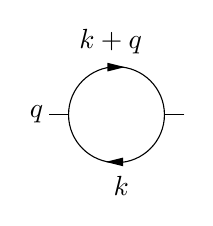
\begin{tikzpicture}[x=0.75pt,y=0.75pt,yscale=-0.7,xscale=0.7]
            %uncomment if require: \path (0,300); %set diagram left start at 0, and has height of 300
            
            %Shape: Circle [id:dp27687562605272853] 
            \draw   (124.71,167) .. controls (124.71,148.77) and (139.48,134) .. (157.71,134) .. controls (175.93,134) and (190.71,148.77) .. (190.71,167) .. controls (190.71,185.23) and (175.93,200) .. (157.71,200) .. controls (139.48,200) and (124.71,185.23) .. (124.71,167) -- cycle ;
            %Straight Lines [id:da44287508502417894] 
            \draw    (163.5,134.25) ;
            \draw [shift={(163.5,134.25)}, rotate = 180] [fill={rgb, 255:red, 0; green, 0; blue, 0 }  ][line width=0.08]  [draw opacity=0] (12,-3) -- (0,0) -- (12,3) -- cycle    ;
            %Straight Lines [id:da6995765588189331] 
            \draw    (156.33,199.5) -- (152.33,199.5) ;
            \draw [shift={(150.33,199.5)}, rotate = 360] [fill={rgb, 255:red, 0; green, 0; blue, 0 }  ][line width=0.08]  [draw opacity=0] (12,-3) -- (0,0) -- (12,3) -- cycle    ;
            %Straight Lines [id:da2952513301761772] 
            \draw    (124.71,167) -- (111,167) ;
            %Straight Lines [id:da19550468559149015] 
            \draw    (204.41,167) -- (190.71,167) ;
            
            % Text Node
            \draw (109,167) node [anchor=east] [inner sep=0.75pt]    {$q$};
            % Text Node
            \draw (177,117) node [anchor=east] [inner sep=0.75pt]    {$k+q$};
            % Text Node
            \draw (168,216) node [anchor=east] [inner sep=0.75pt]    {$k$};            
            \end{tikzpicture}                      
    \end{gathered} = 2 \times (-1) \times  \int \frac{\dd[4]{k}}{(2\pi)^4} \ii G^0_{k} \times \ii G^0_{k+q} \eqqcolon \ii \Pi^0_q,
    \label{eq:normal-interaction-correction}
\end{equation}